\section{Autoencoder}\label{sec:autoencoder}
This section starts with describing the basic philosophy of an autoencoder and
then takes a look at different types of autoencoders.

An autoencoder is a neural network trained to copy its input to its output. It
has a hidden layer \textbf{h} internally that describes a code used to represent
the input. The network can be viewed as being composed of two parts: an encoder
function $\textbf{h} = f(\textbf{x})$ and a decoder producing the reconstruction
$\textbf{r} = g(\textbf{h})$. The general structure of autoencoders can be seen
in Figure \ref{fig:autoencoder}.

If an autoencoder is able to learn to set $g(f(\textbf{x}))=\textbf{x}$
anywhere, it is not particularly useful. Rather, autoencoders are designed to be
unable to learn perfectly how to copy. Usually they are restricted in ways that
only approximately allow them to copy and copy only input that resembles the
training data. Since the model is forced to prioritize which input aspects are
to be copied, it often learns useful data properties. 

For decades, the idea of autoencoders has been part of the neural networks'
historical landscape. Autoencoders have traditionally been used to reduce
dimensionality or to learn features. Recently, autoencoders and latent variable
models have brought autoencoders to the forefront of generative modeling.
Autoencoders can be considered as a special case of feedforward networks and can
be trained with the same techniques, typically minibatch gradient descent after
gradients calculated by back-propagation. 

\begin{figure}[h]
    \centering
    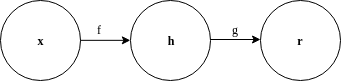
\includegraphics[width=\linewidth]{/1_introduction/autoencoder}
    \caption{An autoencoder's general structure, mapping an input $\textbf{x}$
    to an output (reconstruction) $\textbf{r}$ by an internal representation or
    code $\textbf{h}$. There are two components in the autoencoder: the encoder
    $f$ (mapping $\textbf{x}$ to $\textbf{h}$) and $g$ (mapping $\textbf{h}$ to
    $\textbf{r}$).}
\end{figure}


\subsection{Undercomplete Autoencoders}
Copying the input to the output may sound useless, but we are not usually
interested in the decoder's output. We hope instead that training the
autoencoder to perform the task of copying input will result in h taking on
useful properties.

One way of obtaining useful features from the autoencoder is to limit h to a
smaller size than $\textbf{x}$. An auto encoder is called \textbf{undercomplete} whose
code dimension is less than the input dimension. Learning an undercomplete
representation causes the autoencoder to capture the training data's most
important features. 

The learning process is simply described as minimizing a loss function 
\begin{equation}
    L(\textbf{x}, g(f(\textbf{x}))),
\end{equation}
where L is a loss function that penalizes $g(f(\textbf{x}))$ as being dissimilar
to $\textbf{x}$, such as the mean squared error. 

An undercomplete autoencoder learns to span the same subspace as principal
component analysis (PCA) when the decoder is linear and $L$ is the mean squared
error. In this case, the principal subspace of the training data has been
learned as a side effect by an autoencoder trained to perform the copying task.

Thus, autoencoders with nonlinear encoder functions $f$ and nonlinear decoder
functions $g$ can learn to generalize PCA more powerfully. Unfortunately, if too
much capacity is permitted for the encoder and decoder, the autoencoder can
learn to perform the copying task without extracting useful data distribution
information. 

\subsection{Regularized Autoencoders}
A similar problem occurs when the hidden code has dimensions equal to the input,
and when the hidden code has dimensions larger than the input. In these cases,
even a linear encoder and a linear decoder can learn how to replicate the input
to the output without learning anything meaningful about the distribution of
the data. 

Ideally, any autoencoder architecture could be successfully trained by selecting
the code dimension and the encoder and decoder capacity based on the complexity
of the distribution to be modeled. Regularized autoencoders provide this
ability. Instead of limiting model capacity by keeping the encoder and decoder
shallow and code size small, regularized autoencoders use a loss function that
encourages the model to have other characteristics in addition to being able to
copy its input to its output. These other characteristics include sparsity of
representation, smallness of representation derivative, and robustness to noise
or missing inputs. 

In addition to the methods described here, which are interpreted most naturally
as regularized autoencoders, almost any generative model with latent variables
and equipped with an inference procedure (for computing latent representations
given input) can be considered as a particular form of autoencoder. Variational
autoencoders are another generative modeling approach that emphasizes this
connection with autoencoders. Naturally, these models learn high-capacity,
overcomplete input encodings and do not require regularization to be useful.
Their encoding is naturally effective as the models have been trained to
approximately maximize the probability of training data rather than copying the
input to the output. 

\subsection{Stochastic Encoders and Decoders}
Autoencoders are feedworward networks. The same loss functions and output unit
types thar are used for traditional feedforward networks can be used for
autoencoders aswell.

A general strategy for the design of the output units and the feedforward
network loss function is to define the output distribution
$p(\textbf{y}|\textbf{x})$ and minimize the negative log-likelihood $-\log
p(\textbf{y}|\textbf{x})$ . In that case \textbf{y} is a vector of targets, such
as class labels.

We may think of the decoder as a conditional distribution \\
$p_{decoder}(\textbf{x}|\textbf{h})$ given a hidden code $\textbf{h}$. Then, by
minimizing 
\begin{equation}
    -\log p_{decoder}(\textbf{x}|\textbf{h})
\end{equation}
we can train the autoencoder. The exact shape of this loss function depends on
the shape of \textbf{p}. Additionally, we can generalize the notion of an
\textbf{encoding function} $f(\textbf{x})$ to an \textbf{encoding distribution}
$p_{encoder}(\textbf{h}|\textbf{x})$.

\begin{figure}
	\centering
	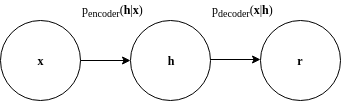
\includegraphics[width=\linewidth]{/1_introduction/autoencoder_stochastic}
    \caption{The architecture of a stochastic autoencoder, in which both the
    encoder and the decoder are not simple functions. Their output can be seen
    as samples from a distribution, $p_{encoder}(\textbf{h}|\textbf{x})$ for the
    encoder and $p_{decoder}(\textbf{x}|\textbf{h})$ for the decoder.} 
	\label{fig:autoencoder}
\end{figure}

\subsection{Variational Autoencoders} \label{subsec:varautoencoders}
Many generative models are based on the idea of using a differentiable generator
network. The model uses a differentiable function that is typically represented
by a neural network to transform samples of latent variables \textbf{z} into
samples \textbf{x} or distributions over samples \textbf{x}. This model class includes
autoencoders that match the generator net with an inference net (encoder).

To generate a sample from the model, the VAE first draws a sample \textbf{z}
from the code distribution $p_{model}(\textbf{z})$. Then the sample runs through
a differentiable generator network $g(\textbf{z})$. At last, \textbf{x} is
sampled from a distribution $ p_{model}(\textbf{x};g(\textbf{z})) =
p_{model}(\textbf{x}|\textbf{z})$. During training, the encoder
$q(\textbf{z}|\textbf{x})$ is used to obtain \textbf{z}, and
$p_{model}(\textbf{x}|\textbf{z})$ is then viewed as decoder network. The
architectural overview of an variational autoencoder can is visualized in
\ref{fig:autoencoder_architecture}.

The key insight behind variational autoencoders is that they can be trained by
maximizing the variational lower bound $\mathcal{L}(q)$ associated with data
point \textbf{x}:

\begin{figure}
	\centering
	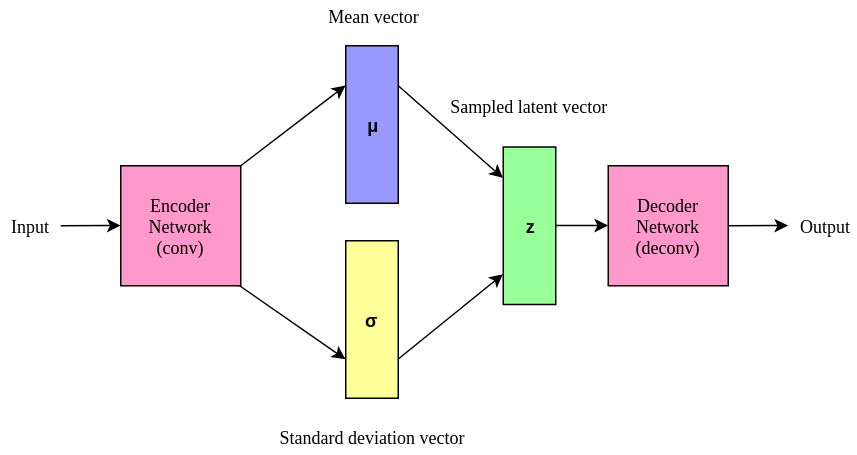
\includegraphics[width=\linewidth]{/2_background/variational_autoencoder_architecture}
    \caption{The architectural overview of a variational autoencoder. On the
    left side is the encoder which is typically a convolutional neural network.
    In the middle we see the standard deviation and the mean of the distribution
    $q(z|x)$ which are optimized during training. Following the with sampled
    latent vector z and the decoder $p_{model}(x|z)$ containing the generator
    network $g(z)$.} 
	\label{fig:autoencoder_architecture}
\end{figure}

\begin{flalign}
    \mathcal{L}(q)  &= \mathds{E}_{z \sim q(\textbf{z}|\textbf{x})} \log p_{model}(\textbf{z}, \textbf{x}) + \mathcal{H}(q(\textbf{z}|\textbf{x})) \label{vae:1} && \\
                    &= \mathds{E}_{z \sim q(\textbf{z}|\textbf{x})} \log 
                    p_{model}(\textbf{x}|\textbf{z}) -
                    D_{KL}(q(\textbf{z}|\textbf{x})||p_{model}(\textbf{z})) \label{vae:2} && \\
                    &\leq \log p_{model}(\textbf{x}).
\end{flalign}

In equation \ref{vae:1}, the first term defines the expected value of the joint
log-likelihood of the visible and hidden variables with respect to the
probabilty distribution $q(\textbf{z}|\textbf{x})$ (approximate posteriror). The
second term defines the entropy of the approximate posterior. The entropy term
encourages the variational posterior to place high probabilty mass on many
\textbf{z} values that could have generated \textbf{x}, rather than collapsing
to a single point estimate of the most likely value.

In equation \ref{vae:2} we recognize the first term as the reconstruction
log-likelihood found in other autoencoders. The second term make the posterior
distribution $q(\textbf{z}|\textbf{x})$ and the model prior
$p_{model}(\textbf{z})$ distribution approach each other. This is accomplished with the
Kullback-Leibler divergence which is a measure of how one probability
distribution is different from a second.

The main idea behind the variational autoencoder is to train an encoder that
produces the parameters of $q$. As long as $\textbf{z}$ is a continuous
variable, it is possible to back-propagate through the samples (by using the
reparameterization trick) of $\textbf{z}$ drawn from $q(\textbf{z}|\textbf{x}) =
q(\textbf{z};f(\textbf{x};\boldsymbol\theta))$ to obtain a gradient with respect
to $\boldsymbol\theta$, where $\boldsymbol\theta$ defines the model parameters
of the VAE.

VAE achieves excellent results and is one of the state-of-the-art generative
modeling approaches. The main disadvantage is that samples from variational
autoencoders trained on images tend to be somewhat blurry. It is not yet known
why this phenomenon occurs. One possibility is that the blurriness is an
instrinsic effect of maximum likelihood.

\subsubsection{Reparameterization trick}
Traditional neural networks perform a deterministic transformation of some input
variables \textbf{z}. When using VAE or other generative models, it is necessary
that neural networks implement a stochastic transformation of \textbf{z}.
However, it is not possible to backpropagate through a stochastic node. One
simple solution is to augment the neural network with extra inputs
$\boldsymbol\epsilon$ that are sampled from a simple probability distribution.
The neural network can then continue to perfrom deterministic computation
internally like computing gradients for training using back-propagation.

As an example let us consider the operation of generating a sample from a VAE.
During training the VAE model draws a sample \textbf{z} from
$q(\textbf{z}|\textbf{x})$, which might be a Gaussian distribution with mean
$\mu$ and variance $\sigma^2$.

\begin{equation}
    z \sim \mathcal{N}(\mu, \sigma^2).
\end{equation}

Because an individual sample of z is produced not by a function, but rather by a
sampling process whose output changes every time we query it, it may seem
counterintuitive to take the derivatives of y with respect to the parameters of
its distribution, $\mu$ and $\sigma^2$. However, we can rewrite the sampling
process as transforming an underlying random value $\epsilon \sim
\mathcal{N}(\epsilon; 0, 1)$ to obtain a sample from the desired distribution:

\begin{equation}
    z = \mu + \sigma * \epsilon.
\end{equation}

Now it is possible to back-propagate through the sampling operation, by
regarding it as a deterministic operation with an extra input $\epsilon$.
Figure \ref{reparam_trick} visualizes the reparameterization trick.

\begin{figure}
	\centering
	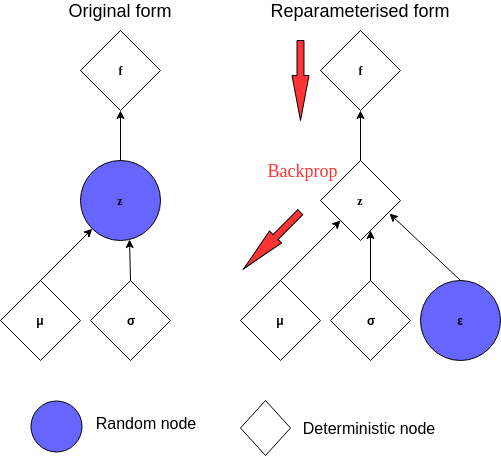
\includegraphics[width=\linewidth]{/2_background/reparam_trick}
    \caption{On the left hand side the original form is displayed. It is not
    possible to back propagate through a stochastic node. On the right side the
    reparameterised form is displayed with a stochastic node $\epsilon$ giving t
    the opportunity to train parameters $\mu$ and $\sigma$ while
    back-propagation.} 
	\label{reparam_trick}
\end{figure}
